\documentclass[12pt,a4paper]{book}

% Load advanced preamble
% ====== Advanced Academic Thesis Preamble ======
% Font and Encoding
\usepackage{fontspec}
\usepackage{unicode-math}
\usepackage{setspace}
\usepackage{parskip}
\usepackage{graphicx}
\usepackage{caption}
\usepackage{subcaption}
\usepackage{xcolor}
\usepackage{microtype}
\usepackage{float}
\usepackage{listings}
\usepackage{tikz}
\newcommand{\code}[1]{\texttt{#1}}
\usetikzlibrary{
    shapes.geometric,
    arrows.meta,
    positioning,
    calc,
    decorations.pathmorphing,
    shadows,
    fit
}
\usepackage{geometry}
\geometry{a4paper, top=1in, bottom=1in, left=1.25in, right=1in}
\onehalfspacing
\setlength{\parskip}{6pt}
\setlength{\parindent}{0pt}

% ===== Colors for Academic Styling =====
\definecolor{RoyalBlue}{RGB}{0,50,150}
\definecolor{SlateGray}{RGB}{100,100,120}
\definecolor{SoftGray}{gray}{0.45}
\definecolor{Highlight}{RGB}{200,30,30} % Optional highlight color

% ===== Section & Chapter Styling =====
\usepackage{titlesec}
\titleformat{\chapter}[display]
  {\normalfont\huge\bfseries\color{RoyalBlue}}
  {\chaptertitlename~\thechapter}{1em}{}
  []  % <-- remove \vspace{1ex}\titlerule

\titleformat{\section}[block]
  {\normalfont\Large\bfseries\color{RoyalBlue}}
  {\thesection}{1em}{}

\titleformat{\subsection}[runin]
  {\normalfont\large\bfseries\color{SlateGray}}
  {\thesubsection}{1em}{}

  
% ===== Fancy Headers & Footers =====
\usepackage{fancyhdr}
\pagestyle{fancy}

% Clear all headers and footers globally
\fancyhf{}
\renewcommand{\footrulewidth}{0pt} % remove footer line

% Header: only for subsequent pages of chapters
\fancyhead[L]{\color{RoyalBlue}\nouppercase{\leftmark}}
\renewcommand{\headrulewidth}{0.4pt}
\renewcommand{\headrule}{\hbox to\headwidth{\color{RoyalBlue}\leaders\hrule height \headrulewidth\hfill}}

% Increase space between header and text content
\setlength{\headsep}{25pt} % adjust as needed

% Remove header on first page of each chapter
\usepackage{etoolbox}
\preto{\chapter}{\thispagestyle{empty}}

% Remove footer entirely
\fancyfoot{}



% Disable headers/footers for frontmatter
\usepackage{etoolbox}
\preto{\chapter}{\thispagestyle{empty}}
\AtBeginEnvironment{abstract}{\thispagestyle{empty}}
\AtBeginDocument{%
    \renewcommand{\chaptermark}[1]{\markboth{#1}{}} % Avoid headers for initial chapters
}

% ===== Hyperlinks =====
\usepackage{hyperref}
\hypersetup{
    colorlinks=true,
    linkcolor=RoyalBlue,
    citecolor=RoyalBlue,
    urlcolor=RoyalBlue,
    pdftitle={Your Thesis Title},
    pdfauthor={Your Name},
    pdfsubject={Thesis Subject},
    pdfkeywords={keyword1, keyword2, keyword3}
}

% ===== Code Listings =====
\usepackage{listings}
\lstset{
    basicstyle=\ttfamily\footnotesize,
    numbers=left,
    numberstyle=\tiny,
    numbersep=5pt,
    frame=single,
    breaklines=true,
    postbreak=\mbox{\textcolor{Highlight}{$\hookrightarrow$}\space},
    keywordstyle=\color{RoyalBlue},
    commentstyle=\color{SoftGray},
    stringstyle=\color{Highlight},
    showstringspaces=false,
    captionpos=b
}

% ===== Bibliography =====
\usepackage[style=ieee, backend=biber]{biblatex}
\addbibresource{18_references.bib}
\DeclareFieldFormat[article,inbook,incollection]{title}{#1}

% Change "Bibliography" to "References"
\DefineBibliographyStrings{english}{
  bibliography = {References},
}

% ===== Glossaries & Acronyms =====
\usepackage[acronym]{glossaries}
\makeglossaries

% ===== Creative Academic Touches =====
% Optional: shaded boxes for definitions or key terms
\usepackage{tcolorbox}
\tcbset{colback=RoyalBlue!5!white, colframe=RoyalBlue, fonttitle=\bfseries}

% ===== Microtype Enhancements =====
\usepackage{microtype}


\begin{document}

% ---------------- FRONTMATTER ----------------
\frontmatter  % Roman page numbers, unnumbered chapters

% Title & Preliminary Pages (No headers)
\thispagestyle{empty}
\begin{titlepage}
    \centering
    
    % University Logo
    
\includegraphics[width=3cm]{logo.jpg}\\[0.5cm]
    
    % University and Department
    {\large \textbf{Addis Ababa Science and Technology University}}\\
    {\large Department of Electrical and Computer Engineering}\\[0.5cm]
    
    % Project Title
    {\Large \textbf{Final Year Project Report}}\\[0.5cm]
    \rule{\textwidth}{1.5pt}\\[0.2cm]
    {\LARGE \textbf{Centralized Ultrasonic-Based Traffic Management System}}\\[0.2cm]
    {\LARGE\textbf{for Speed Limit Violation Detection and Automated Penalty Enforcement}}\\[0.2cm]
    \rule{\textwidth}{1.5pt}\\[1cm]
    
    % Submitted By
    \begin{minipage}{0.9\textwidth}
        \centering
        \textbf{Submitted By:}\\[0.2cm]
        \large
        \begin{tabular}{ll}
            Hiluf Abay & ETS1598/13 \\
            Abdi Fekadu & ETS0002/13 \\
            Bernabas Gebrie & ETS0225/13 \\
            Abdiwak Melaku & ETS0006/13 \\
            Abdulaziz Awol & ETS0008/13 \\
        \end{tabular}
    \end{minipage}\\[1cm]
    
    % Supervisor
    \textbf{Supervisor:}\\[0.2cm]
    \large Mr. Aregawi\\[0.5cm]
    
    % Submission Details
    \textbf{Submitted in Partial Fulfillment of Requirements for}\\[0.2cm]
    \large Bachelor of Science in Electrical and Computer Engineering\\[0.5cm]
    
    % Date
    {\large \textbf{May 2025}}
    
    \vfill
\end{titlepage}
\section*{Declaration}  % The * removes numbering and TOC entry
\addcontentsline{toc}{chapter}{Declaration}  % Add to TOC manually

We, the undersigned, declare that this final year project report titled "Centralized Ultrasonic-Based
Traffic Management System for
Speed Limit Violation Detection and
Automated Penalty Enforcement" is our original work and has not been submitted elsewhere for academic credit.

\vspace{1cm}
\noindent \textbf{Hiluf Abay} \hfill ETS1598/13  \\
\textbf{Abdi Fekadu} \hfill ETS0002/13  \\
\textbf{Bernabas Gebrie} \hfill ETS0225/13  \\
\textbf{Abdiwak Melaku} \hfill ETS0006/13  \\
\textbf{Abdulaziz Awol} \hfill ETS0008/13  

\vspace{1cm}
\noindent \textbf{Supervisor:} Mr.Aregawi

\vspace{1cm}
\noindent \textbf{Date:} May, 2025  

\chapter*{Acknowledgements}
\addcontentsline{toc}{chapter}{Acknowledgements}  % Adds to TOC

First and foremost, we would like to thank Almighty God for granting us the strength, patience, and opportunity to reach this day.

We are deeply grateful to our families for their unwavering love, sacrifices, and belief in us throughout this journey. Their constant support has been the foundation of our perseverance and success.

Our sincere appreciation goes to our supervisor, Mr. Aregawi, for his continuous support, invaluable guidance, and encouragement throughout this project. His insights and feedback have been instrumental in shaping our work.

We also extend our heartfelt thanks to Addis Ababa Science and Technology University for providing us with the necessary resources, facilities, and a conducive learning environment.

\vspace{1cm}
\hfill \textbf{The Authors}

\chapter*{Abstract}
\addcontentsline{toc}{chapter}{Abstract}  % Adds to TOC

This project addresses the growing need for intelligent and automated systems to manage traffic violations, particularly speed limit breaches. It aims to leverage low-cost embedded technologies to detect speed violations, recognize license plate numbers, manage offender data, and automate the fine notification process. The primary objective is to automate speed violation detection and contribute to behavior change among drivers by consistently recording violations and applying penalties.The system uses an ultrasonic sensor for vehicle speed measurement, with an Arduino Uno handling signal processing and speed calibration. A Raspberry Pi, equipped with a camera module, captures images of speeding vehicles. License Plate Recognition (LPR) is achieved using OpenCV and EasyOCR, while SQLite is used for local data storage. Offender notifications are handled through an automated email system using SMTP. Features of the system include speed detection, reliable license plate recognition, and a basic fine system based on the severity of the violation. While the current implementation serves as an academic proof-of-concept, its real-world deployment could significantly enhance traffic law enforcement. It has the potential to reduce accidents caused by overspeeding, minimize corruption by eliminating the need for human traffic officers, and encourage responsible driving by maintaining a record of each driver’s violations.
\tableofcontents
\listoffigures
%\listoftables
\printglossary[type=\acronymtype, title=List of Abbreviations]

% ---------------- MAINMATTER ----------------
\mainmatter  % Arabic page numbers, numbered chapters

% Remove header on first page of each chapter
\preto{\chapter}{\thispagestyle{empty}}


\chapter{Introduction}
Traffic management has become a critical concern in urban areas, particularly in rapidly growing cities like Addis Ababa, Ethiopia. Increasing vehicular traffic, combined with inadequate enforcement of speed limits, poses significant risks to pedestrian safety and public health. Conventional methods of traffic management rely heavily on manual oversight and static measures, often failing to address the dynamic and complex nature of urban traffic violations effectively. Recognizing these challenges, the need for advanced, technology-driven solutions has become evident.
The development of a Centralized Ultrasonic-Based Traffic Management System aims to enhance how traffic violations are monitored and penalized. By leveraging radar technology and centralized control, this system addresses limitations in current practices while offering innovative solutions, such as automated detection of speed limit violations, dynamic fine calculations, and real-time enforcement. This approach not only enhances the accuracy of traffic law enforcement but also contributes to improved road safety, reduced accident rates, and better compliance with traffic regulations.


\section{Background of the Study}
Traffic safety is a pressing issue in Addis Ababa, where pedestrian fatalities account for approximately 80\% of road traffic deaths \cite{unece2021}. Current traffic management methods rely on limited infrastructure, inadequate enforcement, and minimal use of advanced technologies, resulting in significant road safety challenges. Advanced radar-based detection systems, while effective in developed countries, are prohibitively expensive and often incompatible with the financial and infrastructural realities of cities like Addis Ababa.

In Ethiopia, there are no existing radar-based traffic enforcement systems in operation. As a result, traffic law enforcement is predominantly manual, leading to inefficiencies in detecting and addressing violations such as speeding. To fill this gap, a cost-effective, radar-based system tailored to local conditions is essential.

The proposed system seeks to address these challenges by offering an affordable yet efficient solution that combines radar technology with a centralized control system. Unlike high-cost alternatives, this system is designed to be accessible and practical for deployment in Ethiopia, focusing on real-time speed detection, automated fine calculation, and long-term scalability. By prioritizing affordability and leveraging locally available resources, the project aims to revolutionize traffic enforcement while addressing the specific needs of Addis Ababa's road safety landscape.

\section{Statement of the Problem}
Addis Ababa, the capital city of Ethiopia, faces a severe traffic safety crisis primarily driven by high pedestrian fatalities, the impact of speeding, and inadequate traffic management. With a rapidly increasing population and expanding vehicular traffic, road accidents have become a pressing issue significantly affecting public safety. Pedestrians constitute approximately 80\% of all road traffic fatalities in the city \cite{unece2021}. Speeding contributes significantly to accident severity, increasing the risk of injury by up to 3\% and serious injury or death by 5\% with each 1\% increase in average speed \cite{vital2019}. Despite various initiatives to manage traffic, like the 2017 speed management program that reduced average speeds in high-risk areas, more than 90\% of pedestrian deaths still occur at locations without dedicated walkways \cite{wikipedia2021}.

In the fiscal year ending July 2021, Ethiopia recorded 15,034 road accidents, leading to 4,161 deaths \cite{pmid2021}. Many of these accidents can be attributed to poor traffic police management, including insufficient enforcement, lack of proper training, and underreporting of incidents. Research highlights that traffic police in Addis Ababa often lack the necessary qualifications to manage accidents effectively, resulting in significant discrepancies between police-reported traffic deaths and hospital records—153 deaths reported by police compared to 84 recorded in hospitals \cite{acrs2019}. Additionally, drivers’ bad behavior, such as violent conduct and disregard for traffic regulations, remains rampant due to inadequate law enforcement.

The lack of effective traffic police management, combined with poor enforcement and insufficient data-driven approaches, exacerbates the risk of accidents in Addis Ababa. To address this, a centralized ultrasonic-based traffic management system could play a pivotal role in reducing speeding violations, automating penalty issuance, and ultimately improving road safety for both pedestrians and drivers.

\section{Objectives of the Study}

\subsection{General Objective}
To reduce traffic accidents caused by irresponsible drivers speeding in high-risk areas, ensuring safer roads through centralized control, automated enforcement, and dynamic fine systems.

\subsection{Specific Objectives}
\begin{itemize}
  \item Develop a centralized ultrasonic-based traffic management system.
  \begin{itemize}
    \item Integrate the technology speed detection, and violation tracking.
  \end{itemize}
  
  \item Implement a fine system based on speed violations.
  
  \item Enhance the system with automated penalty issuance.
  \begin{itemize}
    \item Automate the process of issuing penalties (warnings, fines, bans) for violations.
  \end{itemize}
  
  \item Implement real-time traffic violation monitoring and reporting.
  \begin{itemize}
    \item Enable continuous monitoring and reporting of traffic violations.
  \end{itemize}
\end{itemize}

\section{Scope of the Study}
The primary focus is on developing an ultrasonic-based system for detecting speeding vehicles and capturing license plate images, with enhancements aimed to streamline data management, and utomating enforcement actions.

\subsection*{1. Hardware Development}
\begin{itemize}
  \item Construction of an ultrasonic circuit capable of accurately detecting vehicle speeds.
  \item Integration of a high-resolution camera to capture images of speeding vehicles.
\end{itemize}

\subsection*{2. Software Development}
\begin{itemize}
  \item Microcontroller programming for real-time speed processing and camera triggering.
  \item Implementation of speed detection algorithms under varying traffic conditions.
  \item License Plate Recognition using OpenCV and EasyOCR with preprocessing techniques.
  \item Integration of a centralized control system using SQLite for tracking and actions.
  \item Email notification via SMTP Simple Mail Transfer Protocol to relevant authorities and systems.
\end{itemize}

\subsection*{3. System Integration}
\begin{itemize}
  \item Combining Arduino, camera, and software modules into a unified system.
  \item Ensuring reliable communication among hardware components and control system.
\end{itemize}

\subsection*{4. Centralized Control System}
\begin{itemize}
  \item The system logs violations over time.
  \item Drivers accumulating a threshold number of violations are flagged for a ban.
  \item All communication and decision-making are automated for transparency and scalability.
\end{itemize}


\chapter{Literature Review}

\section{Theoretical Review of the Literature}

Vehicle speed detection is an essential component of intelligent transportation systems (ITS), contributing to improved traffic management, road safety, and enforcement of legal speed limits~\cite{its_overview}. Several methods have been proposed and implemented for vehicle speed estimation, with ultrasonic sensors and image processing standing out due to their affordability and practical feasibility.

\section*{Ultrasonic Sensor-Based Vehicle Speed Detection}

Ultrasonic sensors function by emitting high-frequency sound waves and measuring the time it takes for the echo to return after reflecting off a nearby object. This time-of-flight (ToF) measurement is used to compute distance. By capturing distance at two distinct time points, the velocity of a moving object can be estimated~\cite{ultrasonic_random_nerd}.

The HC-SR04 ultrasonic sensor is a popular choice in academic and prototype projects because of its low cost, ease of use, and compatibility with microcontrollers like the Arduino. Various implementations have used a pair of ultrasonic sensors placed at a fixed distance to determine vehicle speed based on the time a vehicle takes to pass between them~\cite{ultrasonic_researchgate}. Alternatively, a single sensor aligned with the motion direction can also infer speed by measuring how quickly the object approaches or recedes~\cite{ultrasonic_ieee_paper}.

Despite their practicality, ultrasonic sensors have several limitations:
\begin{itemize}
    \item Limited detection range and narrow beam width
    \item Sensitivity to environmental factors such as temperature, wind, and noise
    \item Inaccurate measurements for small, irregular, or angled objects
\end{itemize}

Nevertheless, for short-range, low-speed environments, ultrasonic sensors are widely regarded as viable solutions~\cite{ultrasonic_instructables}.

\section*{Image Processing-Based Vehicle Speed Detection}

Image processing techniques calculate speed by analyzing vehicle motion across consecutive video frames. This approach involves capturing images, segmenting moving vehicles, and tracking them over time. Given the frame rate and a known real-world reference distance, speed can be computed based on the displacement of the vehicle between frames~\cite{image_processing_speed_detection}.

This method offers distinct advantages, including visual confirmation of events, license plate recognition, and the possibility of integrating AI-based object detection and classification. However, it also introduces challenges such as:
\begin{itemize}
    \item Sensitivity to ambient lighting and adverse weather
    \item Requirements for high-resolution cameras and fixed installations
    \item Greater processing demands for real-time operation
\end{itemize}

Despite these challenges, image-based vehicle speed detection systems remain prevalent, particularly when hardware such as the Raspberry Pi is used to balance computational efficiency and portability.

\section*{License Plate Recognition (LPR)}

License Plate Recognition (LPR) is a specialized form of Optical Character Recognition (OCR) used to identify vehicles based on their license plates from captured images or video frames. It plays a vital role in intelligent transportation systems (ITS) by enabling automated enforcement, vehicle tracking, toll collection, and parking management~\cite{lpr_survey}.

A typical LPR pipeline consists of four main stages:
\begin{enumerate}
    \item {Image Acquisition:} Capturing images or video frames using a camera, typically mounted at an overhead or roadside location.
    \item {License Plate Detection:} Locating the region of interest (ROI) where the license plate exists in the image.
    \item {Character Segmentation:} Isolating individual characters from the plate.
    \item {Character Recognition:} Applying OCR or deep learning methods to interpret segmented characters.
\end{enumerate}

\subsection*{Traditional vs Deep Learning-Based Approaches}

Traditional LPR systems relied heavily on rule-based methods and handcrafted features such as edge detection, morphological operations, and projection profiles for character segmentation and recognition~\cite{traditional_lpr}. While effective under controlled lighting and simple backgrounds, these methods struggled with blurred, tilted, or occluded plates.

Recent advances in deep learning have significantly improved LPR robustness and accuracy. Convolutional Neural Networks (CNNs) and object detection models like YOLO (You Only Look Once) and SSD (Single Shot Detector) have been applied to detect license plates in challenging conditions~\cite{yolo_lpr}. Once the plate is detected, sequence models such as Recurrent Neural Networks (RNNs) or CRNNs (Convolutional Recurrent Neural Networks) are used to recognize characters without explicit segmentation~\cite{crnn_lpr}.

\subsection*{Lightweight Models for Embedded Systems}

For resource-constrained platforms such as the Raspberry Pi, lightweight deep learning models like YOLOv4-tiny and MobileNet-SSD offer real-time performance while maintaining acceptable accuracy~\cite{mobilenet_lpr}. Pretrained models such as `openalpr` and `EasyOCR` are widely adopted due to their ease of integration and high success rates in common scenarios~\cite{easyocr}.

\subsection*{Challenges in LPR}

Despite progress, several challenges persist in LPR:
\begin{itemize}
    \item {Environmental Sensitivity:} Variations in lighting, shadows, weather, and motion blur can significantly affect detection and recognition accuracy.
    \item {Plate Diversity:} Differences in plate formats, fonts, languages, and mounting positions add complexity to general-purpose models.
    \item {Occlusions and Angles:} Obstructed or angled views of plates reduce detection accuracy, particularly for traditional models.
\end{itemize}

By combining LPR with speed violation detection in a modular system, violations can be documented with vehicle identification data, supporting automated enforcement and centralized logging.


\section{Empirical Review}

Recent research has demonstrated the effectiveness of various sensor-based and image-based techniques for vehicle monitoring systems. In particular, ultrasonic sensors have gained traction for short-range, low-power speed detection. For instance,~\cite{ultrasonic_researchgate} implemented a dual-ultrasonic sensor arrangement and demonstrated reliable speed estimation in controlled environments. Likewise,~\cite{ultrasonic_ieee_paper} used a network of ultrasonic transceivers to improve accuracy and classify vehicle types through waveform analysis and reflection timing.

Despite their low cost and energy efficiency, ultrasonic systems face limitations in noisy outdoor environments, especially under conditions involving angled incidence, wind interference, or large vehicle surfaces causing signal dispersion. However, their performance in specific detection zones makes them suitable for triggering events like speed violations.

On the other hand, image-based systems—particularly those leveraging machine learning and optical character recognition (OCR)—are widely used for vehicle identification through License Plate Recognition (LPR). Systems like OpenALPR and EasyOCR have been deployed for detecting and reading license plates under varied lighting and traffic conditions~\cite{lpr_survey, easyocr_github}. These methods often involve multiple stages such as image preprocessing, localization, character segmentation, and recognition.

Studies have shown that LPR systems are sensitive to factors such as motion blur, lighting variations, and low-resolution imagery~\cite{lpr_challenges_paper}. Nevertheless, modern approaches employing convolutional neural networks (CNNs) have improved robustness and character recognition accuracy, even in low-quality frames~\cite{cnn_lpr_improvement}.

Recent works have also explored combining detection and recognition in resource-constrained environments. For instance, lightweight LPR algorithms have been adapted for Raspberry Pi platforms to enable edge computing and real-time traffic monitoring~\cite{raspi_lpr_edge}. These systems benefit from triggering mechanisms to minimize power consumption and unnecessary computation, a principle that aligns well with ultrasonic sensor activation.

\section{Research Gaps}

While both ultrasonic and image processing technologies offer valuable tools for vehicle monitoring, each exhibits limitations when used independently. Ultrasonic sensors, though affordable and power-efficient, provide limited contextual information and are prone to errors due to ambient noise or improper alignment. They are primarily effective at measuring distance or speed in constrained scenarios and offer no means of identifying specific vehicles.

Conversely, image-based systems, especially those used for License Plate Recognition (LPR), are computationally intensive and require high-quality images with consistent lighting. When used continuously, these systems can overwhelm low-power edge devices like the Raspberry Pi. Furthermore, in traffic scenarios with multiple vehicles or occluded views, image-based tracking and recognition become challenging without precise event triggers.

The gap lies in creating a low-cost, hybrid system that balances sensing accuracy, computational efficiency, and reliability. This research proposes a fused approach where an ultrasonic sensor monitors vehicle speed in real time and activates image capture only upon speed threshold violations. The image is then processed using a lightweight LPR algorithm on the Raspberry Pi to extract license plate details and assign penalties. This conditional activation strategy reduces computational overhead, enhances energy efficiency, and optimizes resource usage while maintaining real-time response capability.

By leveraging the strengths of both ultrasonic sensing and image-based recognition, this hybrid architecture addresses individual weaknesses and provides a practical, scalable solution for smart traffic enforcement systems.


\chapter{Methodology}
This chapter outlines the methodological framework employed in the design, development, and evaluation of the \textit{Centralized Ultrasonic Sensor-Based Traffic Management System for Speed Limit Violation Detection and Automated Penalty Enforcement}. The primary objective of this section is to detail the structured and systematic approach used to transform conceptual goals into a functional prototype that accurately detects speed violations and autonomously enforces penalties.

The methodology integrates multiple engineering domains—including ultrasonic signal acquisition, embedded system integration, digital signal processing, and network communication protocols—into a cohesive workflow. Instead of immediately presenting technical implementations, this chapter begins with a high-level overview of the system architecture and proceeds to explain the processing pipeline used to estimate vehicle speed based on time-of-flight (ToF) measurements from ultrasonic sensors.

Subsequent sections elaborate on hardware selection (including Arduino and Raspberry Pi boards), software implementation for real-time speed calculation and license plate recognition, system calibration, and testing procedures. The system uses a threshold-based activation mechanism: when the ultrasonic sensor detects a speed violation, the Raspberry Pi triggers image processing and performs license plate recognition.

\section{Overview of Methodological Approach}
\label{sec:methodology-overview}

The methodological approach adopted in this study follows a modular and sequential framework, where each subsystem contributes to the overall functionality of the centralized ultrasonic-based traffic management system. The process begins with vehicle detection and speed estimation using a single ultrasonic sensor. The system measures the time-of-flight (ToF) of reflected ultrasonic pulses to estimate the distance of a moving vehicle at two successive timestamps. By calculating the change in distance over time, the vehicle's speed is computed in real time.

In parallel, a camera module continuously captures images of approaching vehicles. However, image processing procedures—including license plate recognition—are only initiated if the computed speed exceeds a predefined threshold. This conditional processing reduces computational load on the Raspberry Pi and conserves system resources.

Once the vehicle’s license plate number is extracted, relevant metadata—including speed, timestamp, and license plate number—is appended into a locally hosted SQLite database. This database maintains a historical log of all violations and links repeated offenses to the same vehicle. Upon confirmation of a violation, the system automatically sends an email notification containing the violation details and associated penalty.

This structured methodology ensures a streamlined and resource-efficient integration between sensing, decision-making, and enforcement, making the system scalable, cost-effective, and practical for real-world traffic monitoring applications.


\section{Limitations and Assumptions}

The methodology assumes a direct line-of-sight between the sensor and the target vehicle. It is optimized for single-vehicle detection and may exhibit limitations when multiple moving targets are present simultaneously. Environmental factors such as extreme weather or reflective clutter may affect accuracy.



\section{System Architecture}
\label{sec:system-architecture}
The architecture of the Centralized Ultrasonic-Based Traffic Management System for Speed Limit Violation Detection and Automated Penalty Enforcement is designed as a standalone embedded proof-of-concept solution that integrates sensing, processing, and enforcement functionalities. The system comprises two main processing units: an Arduino microcontroller and a Raspberry Pi single-board computer, each assigned specific roles to ensure efficient operation.

The Arduino interfaces with a single ultrasonic sensor to measure the time-of-flight (ToF) of acoustic pulses reflected by passing vehicles, estimating the distance at two successive time intervals. Using these measurements, the Arduino calculates the vehicle’s speed in real time. This speed data is then transmitted to the Raspberry Pi through GPIO communication.

Meanwhile, the Raspberry Pi continuously captures road images using a Pi Camera Module. However, image processing—including license plate recognition via OpenCV and EasyOCR—is initiated only when the speed received from the Arduino exceeds the predefined speed limit. This conditional approach minimizes unnecessary computation, thereby optimizing system performance.

Once a speeding violation is detected, the Raspberry Pi performs license plate number (LPN) extraction. Subsequently, the extracted LPN is used to filter driver information from a hardcoded lookup table containing details such as the driver’s name, email address, and status. The system then records the violation—including speed, timestamp, and license plate number—in a locally hosted SQLite database.

Finally, an automated email notification is generated and sent to the offending driver. This email contains details of the violation, including the fine amount and the reason for the penalty. The violation record is updated accordingly to reflect the enforcement action.

This modular design ensures clear separation of low-level sensing tasks and high-level processing and decision-making, enabling scalable integration with centralized traffic management systems or cloud-based analytics platforms in future developments.
.
\begin{figure}[htbp]
    \centering
    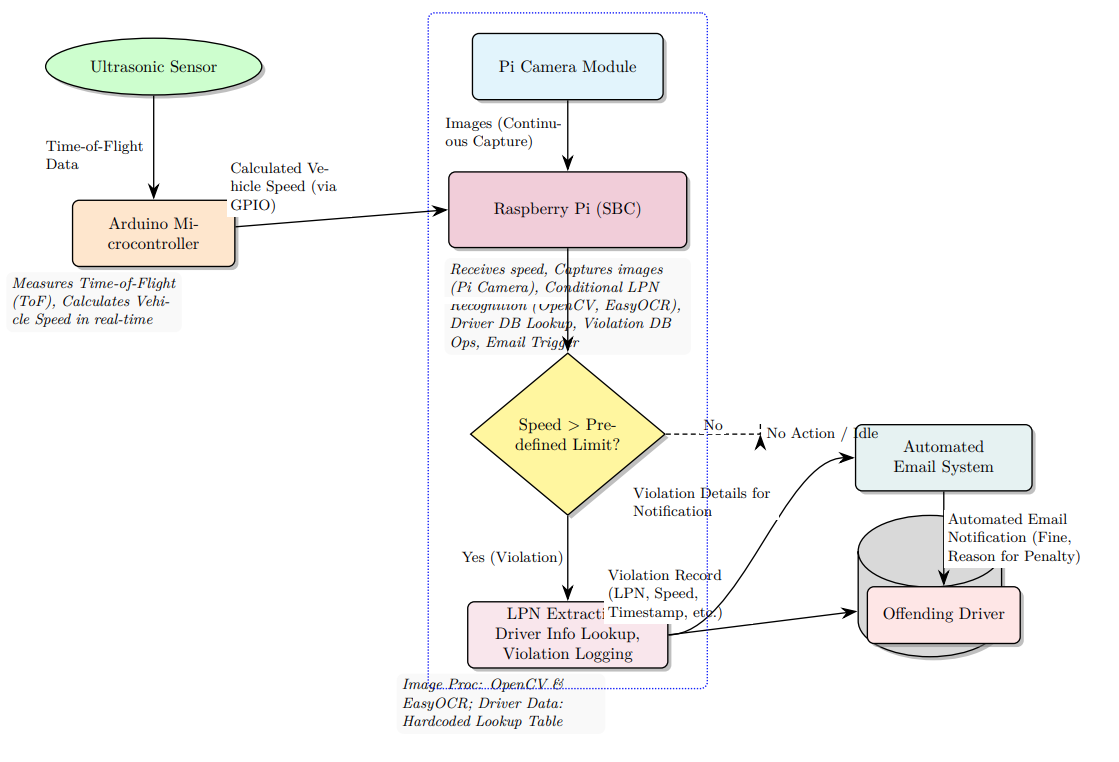
\includegraphics[width=1.0\textwidth]{figures/system_architecture_diagram.png}
    \caption{System architecture diagram}
    \label{fig:system_arch}
\end{figure}

\section{Ultrasonic-Based Speed Detection Module}
\label{sec:ultrasonic-speed-detection}

\subsection*{Principle of Ultrasonic Time-of-Flight Ranging}
Ultrasonic range measurement relies on the time-of-flight (ToF) of high-frequency acoustic pulses between an emitter and a reflecting surface. The sensor emits a short burst of ultrasonic sound (typically around 40~kHz), which propagates through the air at the local speed of sound $c$. When the pulse encounters a vehicle, it reflects back to the sensor's receiver. By measuring the round-trip time $t$, the distance $d$ to the vehicle is computed as:


\begin{equation}
  d = \frac{c \times t}{2}
  \label{eq:tof_distance}
\end{equation}

\begin{figure}[htbp]
  \centering
  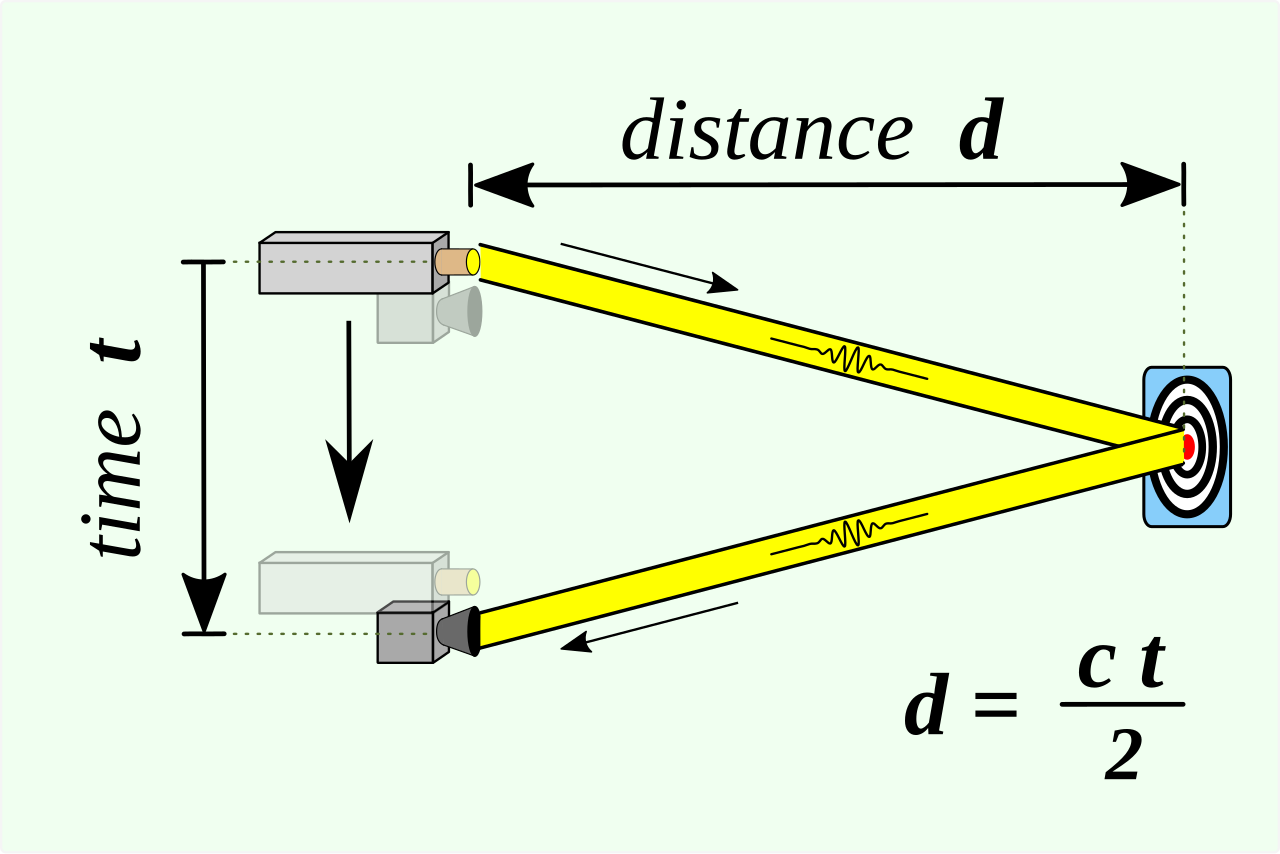
\includegraphics[width=0.8 \linewidth]{figures/ultrasonic.png}
    \caption{HC-SR04 Ultrasonic Sensor for Distance and Speed Estimation}
  \label{fig:ultrasonic-sensor}
\end{figure}


Because the speed of sound in dry air at 20~°C is approximately 343~m/s—and varies by roughly 0.6~m/s for each °C change—many implementations include temperature compensation to maintain accuracy in different environmental conditions.\cite{smith2020ultrasonic}

To determine vehicle speed, the system takes two distance measurements $d_1$ and $d_2$ at times $t_1$ and $t_2$, respectively. Assuming straight-line motion and negligible acceleration between samples, the average speed $v$ over the interval $\Delta t = t_2 - t_1$ is:

\begin{equation}
  v = \frac{d_1 - d_2}{\Delta t}
  \label{eq:speed_estimation}
\end{equation}
In practice, the Arduino microcontroller triggers the ultrasonic sensor at fixed intervals (every 50~ms), computes $d$ for each pulse, and then calculates $v$ in real time. This approach yields a continuous stream of speed data without requiring Doppler processing hardware.\cite{johnson2019measuring}

\subsection*{Implementation of HC-SR04 Ultrasonic Sensor}
The HC-SR04 ultrasonic ranging module is widely used for short-range distance measurement in embedded systems due to its affordability, reliability, and ease of interfacing with microcontrollers. It operates on the principle of ultrasonic time-of-flight (ToF) and provides digital timing signals corresponding to the round-trip duration of an ultrasonic pulse.

\subsubsection{Sensor Architecture and Signal Timing}
The HC-SR04 integrates an ultrasonic transmitter and receiver into a single compact unit. The measurement cycle begins when the microcontroller sends a 10~µs HIGH pulse to the sensor's \texttt{TRIG} (trigger) pin. This pulse initiates the emission of an 8-cycle burst of 40~kHz ultrasonic waves from the transmitter. Simultaneously, the sensor begins timing the echo signal.

These waves propagate through the air until they encounter a reflective object (e.g., a vehicle). The reflected wave is then captured by the receiver. Upon detecting the echo, the sensor pulls the \texttt{ECHO} pin HIGH for a duration proportional to the total round-trip time $t$ of the pulse.

The host microcontroller reads this duration $t$ in microseconds (µs), and the distance $d$ to the target is calculated using:
\begin{equation}
  d = \frac{c \times t}{2}
  \label{eq:hc_distance_eq}
\end{equation}
where $c$ is the speed of sound in air (typically 343~m/s at 20~\textdegree C), and the division by 2 accounts for the round-trip nature of the signal. In practical terms, this is often converted to a simplified empirical formula in centimeters:
\begin{equation}
  d~[\text{cm}] = \frac{t~[\mu s]}{58}
  \label{eq:empirical_cm}
\end{equation}
This approximation assumes $c = 343$~m/s and simplifies real-time processing on microcontrollers like Arduino.

\subsubsection{Speed Estimation Methodology}
To measure the speed of a moving vehicle, the sensor records two consecutive distance readings $d_1$ and $d_2$ at timestamps $t_1$ and $t_2$, respectively. Assuming uniform linear motion between these two readings, the average speed $v$ can be calculated as:
\begin{equation}
  v = \frac{d_1 - d_2}{t_2 - t_1}
  \label{eq:hc_speed}
\end{equation}
The sensor is typically polled at fixed intervals $\Delta t = t_2 - t_1$ (e.g., 50~ms), determined by the microcontroller’s timing logic. Using this periodic sampling, the Arduino continuously computes the instantaneous speed of the object in real-time. A positive value of $v$ indicates motion toward the sensor, while a negative value implies recession.

\subsubsection{Arduino-Based Implementation}
The following high-level steps summarize the software implementation of the HC-SR04 with an Arduino:
\begin{enumerate}
  \item \textit{Trigger Emission}: Set the \texttt{TRIG} pin HIGH for 10~µs to generate an 8-cycle burst.
  \item \textit{Echo Measurement}: Wait for the \texttt{ECHO} pin to go HIGH, and measure the duration $t$ it remains HIGH.
  \item \textit{Distance Calculation}: Convert the duration $t$ to distance using Equation~\ref{eq:empirical_cm}.
  \item \textit{Speed Estimation}: Store successive distance measurements and apply Equation~\ref{eq:hc_speed}.
\end{enumerate}

\subsubsection{Measurement Range and Accuracy}
The HC-SR04 is rated for distances between 2~cm and 400~cm, with typical resolution around ±3~mm under ideal conditions. However, factors such as temperature, humidity, and reflective surface characteristics can introduce errors. Temperature compensation is thus crucial for applications requiring high accuracy. Since the speed of sound $c$ varies approximately by 0.6~m/s per 1~\textdegree C change in air temperature, some implementations use a temperature sensor to adjust $c$ in Equation~\ref{eq:hc_distance_eq}.
\begin{equation}
  c = 331.4 + 0.6T
  \label{eq:temp_compensation}
\end{equation}
where $T$ is the ambient temperature in degrees Celsius.

\subsubsection*{System Integration and Real-Time Considerations}
In the implemented vehicle speed detection system, the HC-SR04 ultrasonic sensor is mounted at a fixed roadside position with an unobstructed line of sight toward approaching vehicles. The Arduino microcontroller manages the emission and reception of ultrasonic pulses at regular intervals, allowing it to compute the speed of passing vehicles in real time. Once a speed value is calculated, it is transmitted to the Raspberry Pi through the serial communication interface. Upon receiving this data, the Raspberry Pi evaluates whether the measured speed exceeds a predefined speed limit. If so, it initiates the image capture process and proceeds with license plate recognition to identify the violating vehicle.

\begin{figure}[htbp]
    \centering
    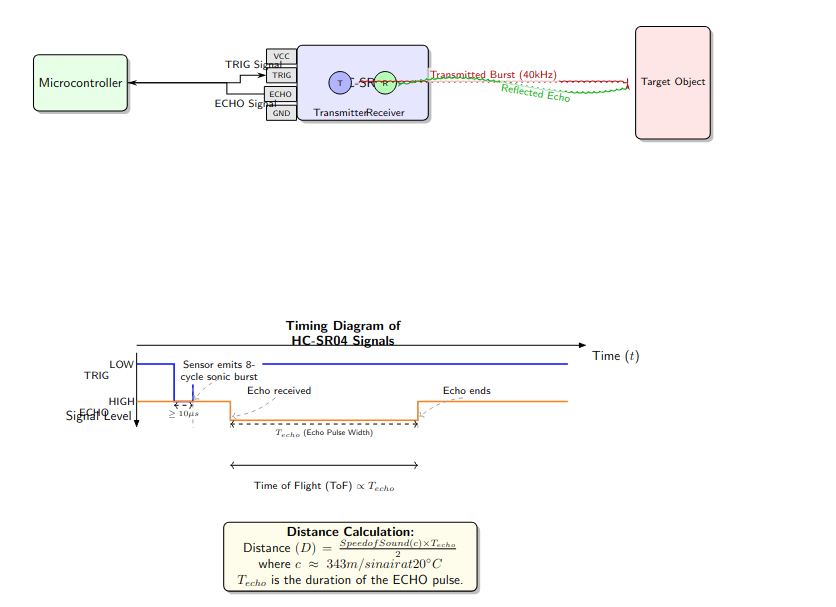
\includegraphics[width=1.0\textwidth]{figures/HC-SR04.png}
    \caption{HC-SR04 Working Principle (Detailed)}
    \label{fig:hc-sr04-detailed}
\end{figure}

\newpage
\subsection*{Advantages and Limitations}
Ultrasonic ToF-based speed detection offers:
\begin{itemize}
  \item {Simplicity and low cost}: Minimal signal processing and inexpensive hardware.
  \item {Robustness}: Works in low-light and varied weather conditions where optical sensors may fail.
\end{itemize}
However, it is subject to:
\begin{itemize}
  \item {Environmental sensitivity}: Variations in temperature, humidity, and wind can affect the speed of sound and introduce errors if uncompensated.
  \item {Beam divergence}: Wide acoustic beams may reflect off unintended surfaces (e.g., ground or nearby structures), requiring careful sensor placement and signal filtering.
\end{itemize}
By understanding these trade-offs, the ultrasonic module can provide reliable speed measurements for triggering downstream license-plate recognition and penalty enforcement in an embedded traffic management system.



\section{Image Capture and License Plate Recognition (LPR)}

This section details the technical methodology employed for the development of the License Plate Recognition (LPR) system, encompassing the hardware setup for image acquisition and the intricate software pipeline for license plate localization and character recognition.

\subsection{Image Acquisition Subsystem}
\label{subsec:image_acquisition}

The image acquisition subsystem is responsible for capturing high-resolution visual data of vehicles, which serves as the primary input for the LPR process.

\subsubsection{Hardware Components}
\label{subsubsec:hardware}

\begin{itemize}
    \item \textbf{Raspberry Pi:} The \textbf{Raspberry Pi 3 Model B+} (with 1GB LPDDR2 SDRAM) serves as the embedded computing platform. Its Broadcom BCM2837B0, Cortex-A53 (ARMv8) 64-bit SoC operating at 1.4GHz provides sufficient processing power for on-device image processing tasks, minimizing latency. The integrated General-Purpose Input/Output (GPIO) pins facilitate direct interfacing with the camera module.
    \item \textbf{Raspberry Pi Camera Module:} Image capture is performed by the \textbf{Raspberry Pi Camera Module V2}. This 8-megapixel camera, featuring a Sony IMX219 sensor, is connected via the dedicated CSI (Camera Serial Interface) port, ensuring high-bandwidth data transfer. The camera is configured to capture still images at a resolution of 720*640 pixels, which provides ample detail for subsequent license plate analysis.

\end{itemize}

\subsubsection{Image Capture Mechanism}
\label{subsubsec:capture_mechanism}

In our implementation, the Raspberry Pi continuously captures still images at fixed time intervals, rather than waiting for an external trigger. Specifically, the camera module is programmed to acquire a high-resolution frame (720×1640 px JPEG) every 100 ms (10 Hz) using a simple loop and the Picamera2 API. Each capture is immediately timestamped and stored—in a directory structured by date and time—to guarantee chronological ordering and ease of retrieval. As soon as an image is written to disk, it is pushed into the OpenCV/EasyOCR processing pipeline for license‐plate localization and character recognition. By decoupling acquisition from motion detection, this periodic sampling approach ensures that no vehicle passing through the sensing zone goes unrecorded, while still bounding CPU and I/O usage by limiting the frame rate to a level that our hardware can sustain in real time..

\subsection*{License Plate Recognition Algorithm}
\label{subsec:lpr_algorithm}

The core of the LPR system is a multi-stage software algorithm implemented primarily in Python, leveraging the \code{OpenCV} and \code{EasyOCR} libraries. The algorithm sequentially processes the captured image to localize the license plate and subsequently recognize its alphanumeric characters.

\begin{figure}[htbp]
    \centering
    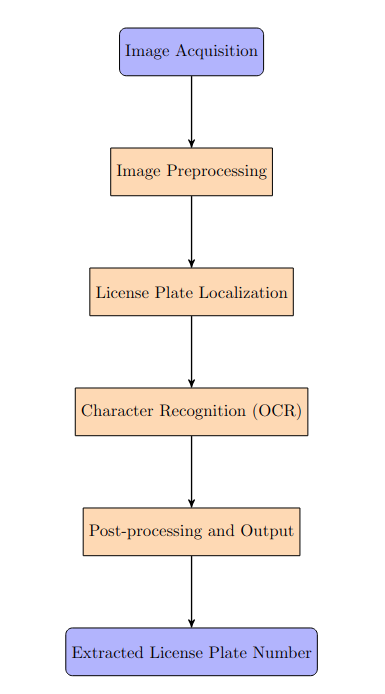
\includegraphics[width=0.95 \textwidth]{figures/LPR.png}
    \caption{ Flowchart of the License Plate Recognition (LPR) Algorithm}
    \label{fig:lpr-flow-chart}
\end{figure}


\subsubsection{Image Preprocessing}
\label{subsubsec:preprocessing}

The initial step involves transforming the raw captured image into a format suitable for robust feature extraction and analysis.

\begin{itemize}
    \item \textbf{Grayscale Conversion:} The 3-channel RGB image is converted to a single-channel grayscale image using \code{cv2.cvtColor(image, cv2.COLOR\_BGR2GRAY)}. This reduces computational complexity by focusing solely on intensity variations, which are critical for edge detection.
    \item \textbf{Noise Reduction:} A \textbf{Gaussian blur} filter is applied to the grayscale image using \code{cv2.GaussianBlur(image, (5, 5), 0)}. This operation smooths the image, reducing high-frequency noise and mitigating the impact of minor imperfections or illumination variations, thereby preventing spurious edges in subsequent steps.
    \item \textbf{Contrast Enhancement:} To improve the distinction between license plate characters and their background, especially under non-uniform lighting, Adaptive Histogram Equalization (AHE), specifically \textbf{Contrast Limited Adaptive Histogram Equalization (CLAHE)}, is applied. This is implemented via \code{cv2.createCLAHE(clipLimit=2.0, tileGridSize=(8,8))} followed by \code{apply()}. CLAHE enhances local contrast without over-amplifying noise in homogeneous regions.
\end{itemize}

\subsubsection{License Plate Localization}
\label{subsubsec:localization}

This stage aims to accurately identify and extract the rectangular region containing the license plate from the preprocessed image.

\begin{itemize}
    \item \textbf{Edge Detection:} The \textbf{Canny edge detector} is applied to the contrast-enhanced grayscale image using \code{cv2.Canny(image, 100, 200)}. This algorithm identifies strong intensity gradients, effectively highlighting potential boundaries of objects, including the license plate and its characters. The thresholds (100 and 200) are empirically determined to balance sensitivity and noise suppression.
    \item \textbf{Morphological Operations:} To connect fragmented edges and enhance the rectangular shape of the license plate, a sequence of morphological operations is performed:
    \begin{itemize}
        \item \textbf{Dilation:} \code{cv2.dilate(edges, kernel, iterations=1)} is applied to thicken the edges and close small gaps, using a rectangular kernel.
        \item \textbf{Erosion:} \code{cv2.erode(dilated\_edges, kernel, iterations=1)} is then applied to thin the thickened edges, effectively removing small noise components while preserving the connected larger structures. This `dilate` then `erode` sequence is equivalent to a \textbf{closing} operation, which is effective at closing small holes and connecting nearby features.
    \end{itemize}
    \item \textbf{Contour Detection and Filtering:}
    \begin{itemize}
        \item \textbf{Contour Finding:} Contours (continuous curves joining all continuous points along the boundary, having the same color or intensity) are detected using \code{cv2.findContours(processed\_edges, cv2.RETR\_LIST, cv2.CHAIN\_APPROX\_SIMPLE)}.
        \item \textbf{Contour Approximation:} Each detected contour is approximated to a simpler polygon using \code{cv2.approxPolyDP(contour, epsilon, True)}, where $\epsilon$ is a small fraction of the contour perimeter. This helps in identifying rectangular shapes more robustly.
        \item \textbf{Filtering by Geometric Properties:} Candidate contours are rigorously filtered based on their geometric properties, which are characteristic of standard license plates:
        \begin{itemize}
            \item \textbf{Area:} Contours with an area (\code{cv2.contourArea}) outside a predefined range (e.g., $A_{\text{min}} \le A \le A_{\text{max}}$) are discarded.
            \item \textbf{Aspect Ratio:} The aspect ratio ($AR = \frac{\text{width}}{\text{height}}$) of the bounding rectangle (\code{cv2.boundingRect}) of each contour is calculated. Typical license plates exhibit an aspect ratio within a specific range, e.g., $2.5 \le AR \le 5.0$ for standard single-line plates.
            \item \textbf{Number of Vertices:} Only contours that, after approximation, have exactly four vertices are considered, indicating a rectangular shape.
            \item \textbf{Solidity:} The ratio of the contour area to the area of its convex hull (\code{cv2.contourArea(cv2.convexHull(contour))}) is checked to ensure the contour is solid and not excessively concave.
        \end{itemize}
    \end{itemize}
    \item \textbf{Region of Interest (ROI) Extraction and Perspective Correction:} The contour that best satisfies all filtering criteria is identified as the license plate. Its bounding box coordinates are extracted. If the license plate is captured at an angle, a perspective transformation is applied to rectify the ROI. This involves:
    \begin{itemize}
        \item Identifying four corner points of the detected license plate.
        \item Defining the corresponding desired output points for a rectified, front-parallel view.
        \item Computing the perspective transformation matrix using \code{cv2.getPerspectiveTransform(src\_points, dst\_points)}.
        \item Applying the transformation to the original image using \code{cv2.warpPerspective(image, M, output\_size)} to obtain a normalized, frontal view of the license plate.
    \end{itemize}
\end{itemize}

\subsubsection{Character Recognition (Optical Character Recognition - OCR)}
\label{subsubsec:ocr}

The localized and rectified license plate ROI is then passed to the OCR engine for character extraction.

\begin{itemize}
    \item \textbf{EasyOCR Integration:} The \code{EasyOCR} library is utilized for this stage. It is initialized with the desired language models (e.g., \code{reader = easyocr.Reader(['en'])} for English).
    \item \textbf{Deep Learning Model:} EasyOCR leverages a combination of deep learning architectures:
    \begin{itemize}
        \item \textbf{Convolutional Recurrent Neural Network (CRNN):} This component extracts features from the image. The Convolutional Neural Network (CNN) layers extract spatial features, which are then fed into Recurrent Neural Network (RNN) layers (specifically, Bidirectional LSTMs) to capture sequential dependencies between features, crucial for recognizing characters in a sequence.
        \item \textbf{Connectionist Temporal Classification (CTC):} This is a loss function used to train recurrent neural networks for sequence labeling problems where the alignment between the input and output sequences is unknown. CTC allows EasyOCR to recognize entire character sequences without explicit segmentation of individual characters, making it robust to variations in character spacing and font.
    \end{itemize}
    \item \textbf{Recognition Output:} The \code{reader.readtext(roi\_image)} function processes the license plate ROI and returns a list of detected text boxes, each containing the recognized text, its bounding box, and a confidence score.
\end{itemize}

\subsubsection{Post-processing and Output}
\label{subsubsec:postprocessing}

The raw OCR output undergoes a final stage of refinement to ensure accuracy and adherence to expected license plate formats.

\begin{itemize}
    \item \textbf{Text Concatenation:} If EasyOCR returns multiple text boxes for a single plate (e.g., due to slight gaps), these are concatenated into a single string, respecting their horizontal order.
    \item \textbf{Regular Expression Filtering:} A regular expression is applied to the recognized string to filter out non-alphanumeric characters and enforce specific patterns typical of license plates in the target region (e.g., `$$[A-Z]{2,3}[0-9]{3}[A-Z]{2}$$` for a hypothetical format). This helps in removing noise and standardizing the output.
    \item \textbf{Error Correction Heuristics:} Common OCR errors (e.g., 'O' vs. '0', 'I' vs. '1', 'S' vs. '5', 'B' vs. '8') are addressed using a set of predefined substitution rules or a lookup table based on common character ambiguities and regional license plate patterns. For instance, if a character 'O' is detected in a position typically reserved for numbers, it might be corrected to '0' based on context.
    \item \textbf{Final Output:} The cleaned and validated alphanumeric string representing the license plate number is then output by the system. This output can be stored in a database, displayed on a user interface, or used to trigger further actions (e.g., gate opening).
\end{itemize}




\section{ Violation Handling and Penalty Enforcement}

Once a license-plate has been recognized and the measured speed \(v\) exceeds the predefined threshold \(v_{\mathrm{lim}}\), the system proceeds with storing the violation and notifying the offending driver. This process is implemented via a lightweight SQLite database and an automated email module, as described below.

\subsubsection{Database Schema and Initialization}
A local SQLite database (\texttt{speed\_monitor.db}) is used to persist driver records and violation events. Two tables are created at startup:
\begin{itemize}
  \item \textbf{drivers}: stores  
    \(\{\)\,id, name, license\_plate, email, violation\_count, created\_at\(\}\).  
    Each driver’s license plate is enforced as unique, and \texttt{violation\_count} tracks the cumulative number of recorded offenses.
  \item \textbf{violations}: stores  
    \(\{\)\,id, driver\_id, speed, timestamp, image\_path\(\}\).  
    A foreign key \texttt{driver\_id} references the \texttt{drivers} table.
\end{itemize}
This schema ensures referential integrity and supports efficient querying of both individual driver histories and aggregate statistics.

\subsubsection{Recording a Violation}
When a new violation is detected, the following steps occur:
\begin{enumerate}
  \item \emph{Driver lookup}: retrieve the driver’s record by matching the recognized license plate.  
  \item \emph{Insert violation}: create a new entry in \texttt{violations} with the fields  
    \(\{\)driver\_id, speed, timestamp, image\_path\(\}\).  
  \item \emph{Increment counter}: update the corresponding driver’s \texttt{violation\_count} by \(+1\).
  \item \emph{Commit transaction}: ensure both tables remain consistent by committing the changes atomically.
\end{enumerate}

\subsubsection{Automated Penalty Notification}
Immediately after persisting the violation, the system constructs and sends an email notification to the driver:
\begin{enumerate}
  \item Query the \texttt{drivers} table to obtain the driver’s name and email.
  \item Generate an email containing:
    \begin{itemize}
      \item Date and time of the violation
      \item Recorded speed and applicable speed limit
      \item Amount of the fine and instructions for payment
    \end{itemize}
  \item Dispatch the message via the \texttt{EmailSender} module using SMTP, embedding a link to the stored image for verification.
\end{enumerate}

\subsubsection{Reporting and Analytics}
The database manager also provides methods to retrieve:
\begin{itemize}
  \item The most recent \(N\) violations, with associated driver names and image paths.
  \item The Top \(M\) speeders, ranked by \texttt{violation\_count}, for enforcement prioritization.
  \item A complete list of registered drivers, including their cumulative violation counts and registration timestamps.
\end{itemize}
These queries support both real-time dashboard displays and offline analysis of traffic patterns and repeat offenders.

---

By centralizing all violation data in an embedded SQLite database and linking it to an automated email notification system, the implementation ensures that every detected offense is reliably recorded, the driver is promptly informed, and historical data can be mined for policy or system-tuning purposes.```





\chapter{Implementation}

\section{System Overview}
This section provides a high-level summary of the hardware and software components implemented in the vehicle speed detection and penalty enforcement system. The architecture integrates an Arduino-based ultrasonic module for speed measurement and a Raspberry Pi-based framework for image capture, license plate recognition, violation recording, and notification.

\section{Hardware Implementation}

\subsection{Ultrasonic Speed Measurement (Arduino)}
The HC-SR04 ultrasonic sensor is mounted perpendicular to the roadway at a height of 5cm. The Arduino measures vehicle speed using two successive time-of-flight (ToF) readings separated by a fixed physical interval. Calculated speed values are transmitted via serial comm. USB to the Raspberry Pi. Detailed operation:
\begin{enumerate}
  \item Trigger a 40~kHz ultrasonic burst via the TRIG pin (10~\textmu s HIGH).
  \item Measure the echo pulse duration on the ECHO pin to compute distance using Equation~\eqref{eq:hc_distance_eq}.
  \item Estimate speed by differencing successive distances over a fixed time interval (50~ms).
  \item Output a digital to Raspberry Pi.
\end{enumerate}

\subsection{Raspberry Pi Camera Setup}
A Raspberry Pi Camera Module V2 is configured via the \texttt{picamera2} library to capture 1280\,$\times$\,720 JPEG frames at 10~Hz. Images are stored in a timestamped directory structure for subsequent processing.

\section{Software Implementation}
\subsection*{Software Implementation on Arduino}

The Arduino is programmed to measure the speed of approaching vehicles using a single ultrasonic sensor (HC-SR04) and to communicate with the Raspberry Pi when a speed violation is detected. The key responsibilities of the Arduino code are to perform distance measurements, compute real-time speed, display results on an LCD, and trigger an alert to the Raspberry Pi in the event of a speeding violation.

\subsubsection*{Libraries Used}

To simplify the implementation, the following libraries were used:

\begin{itemize}
    \item \texttt{HCSR04.h}: Facilitates precise distance measurement using the HC-SR04 ultrasonic sensor.
    \item \texttt{Wire.h}: Supports I\textsuperscript{2}C communication, which is essential for interfacing with the LCD.
    \item \texttt{LiquidCrystal\_I2C.h}: Manages the 16x2 LCD display using the I\textsuperscript{2}C interface, reducing the number of GPIO pins required.
\end{itemize}

\subsubsection*{Measurement and Display Logic}

The Arduino performs multiple ultrasonic distance readings in quick succession and computes an average to improve reliability and reduce the impact of sensor noise. Speed is calculated using the difference between successive distance measurements divided by the time elapsed. The result, initially in cm/s, is converted to km/h and displayed on a 16x2 LCD screen alongside the distance.

To prevent erratic readings, the code includes filtering logic such as range validation and minimum update intervals. This ensures that only valid, stable measurements are used in the computation.

\subsubsection*{Speed Violation Detection and Signaling}

When the computed speed exceeds a predefined threshold , a GPIO pin on the Arduino is toggled HIGH for a short duration to signal the Raspberry Pi. This serves as an interrupt-style alert for further processing. A debounce mechanism is included to prevent repeated signals within a short timeframe, ensuring each event is uniquely recognized and handled.

\subsubsection*{Code and Circuit Layout}

The complete Arduino code and the corresponding Proteus simulation layout used for testing and validation are provided in \textbf{Appendix A}.

\section{Software Implementation: License Plate Recognition System}

This section presents the software implementation of the License Plate Recognition (LPR) system, a core component of the overall speed monitoring solution. The system is designed to automatically detect and read vehicle license plates, particularly for those that exceed a predefined speed limit, and log relevant violation data. The software architecture follows a modular design, comprising components for image acquisition, license plate processing, violation management, and automated notification.

\subsubsection*{Production Environment (Raspberry Pi)}

For the deployment phase, the Raspberry Pi serves as the host platform. The system utilizes the \texttt{picamera2} library to interface with the Pi camera module. The camera is configured to capture high-resolution images at 1920$\times$1080 pixels, which are then passed to the image processing pipeline.


\subsection{License Plate Processing Module}

At the core of the LPR system lies its capability to extract license plate information from images. The processing workflow comprises several stages:

\subsubsection{Preprocessing}

Captured images are first converted to grayscale, followed by the application of a Gaussian blur. These operations are essential for reducing noise and enhancing salient features needed for reliable license plate detection.

\subsubsection{Feature Extraction}

The Canny edge detection algorithm is applied to the preprocessed images to identify object boundaries. This aids in highlighting potential license plate regions.

\subsubsection{Region of Interest (ROI) Identification}

Contours are extracted from the edge-detected image. These contours are evaluated based on geometric properties, particularly aspect ratio, which helps isolate regions likely to contain license plates.

\subsubsection{Optical Character Recognition (OCR)}

Once a candidate license plate region is identified, the system uses the \texttt{easyocr} library to perform OCR. This converts the visual characters within the image to machine-readable text. The OCR engine is configured to recognize English alphanumeric characters.

\subsection{Speed Monitoring and Violation Management Module}

This module integrates real-time speed monitoring with the LPR component to manage speed limit violations.

\subsubsection{Speed Detection Integration}

In the production environment, speed data is received via a serial USB on the Raspberry Pi. For development and testing, speed values are simulated.

\subsubsection{Thresholding and Triggering}

A speed threshold (20.0 m/s) is defined. When a vehicle's measured speed exceeds this limit, the system triggers the violation logging process.

\subsubsection{Violation Logging}

Upon detecting a violation, the system logs the following information:
\begin{itemize}
    \item Timestamp of the event,
    \item Measured vehicle speed,
    \item Extracted license plate number,
    \item Captured image of the vehicle.
\end{itemize}
These data points are stored in a centralized database for analysis and future reference.

\subsubsection{Automated Notification}

An automated notification mechanism is implemented. The system queries the database for driver profiles corresponding to the detected license plate. If a match is found and an email address is available, an email notification is automatically dispatched, including violation details and the image of the vehicle.

For further details about the codes, refer Appendix B and C.

\chapter{Results and Discussion}

\section{Overview of Testing Environment}
The system was tested in both development and production environments. The development environment utilized a Pi camera and simulated speed values, allowing flexible testing of software components. The production environment employed a Raspberry Pi with PiCamera and an Arduino Uno with an ultrasonic sensor (HC-SR04) for real-world deployment. All modules were integrated and tested in a controlled indoor setting to simulate vehicle motion.

\section{Speed Detection Results}
The speed detection module calculates speed by measuring the time taken for a vehicle to travel a fixed distance using ultrasonic sensing. 

\begin{figure}[!htbp]
\centering
\begin{subfigure}[b]{0.48\textwidth}
\centering
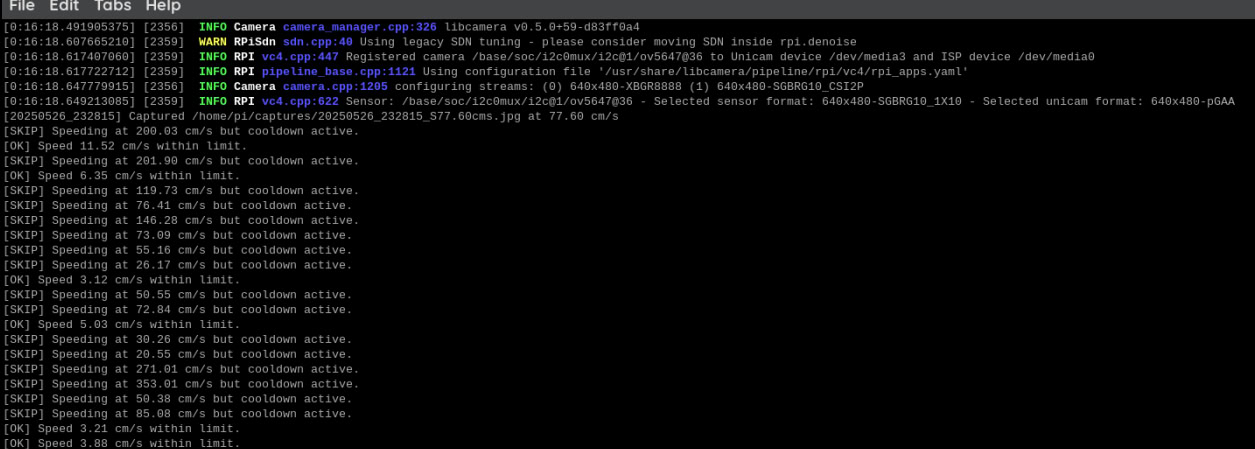
\includegraphics[width=\textwidth]{figures/photo_2025-05-27_01-24-17.jpg}
\caption{Speed violation detection scenario}
\label{fig:violation}
\end{subfigure}
\hfill
\begin{subfigure}[b]{0.48\textwidth}
\centering
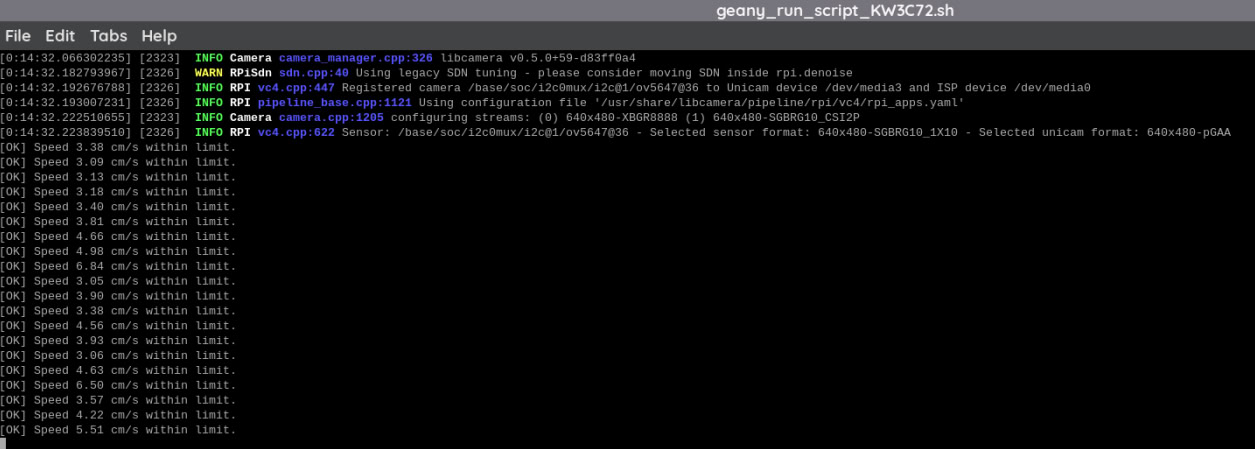
\includegraphics[width=\textwidth]{figures/photo_2025-05-27_01-24-10.jpg}
\caption{Normal operation scenario}
\label{fig:normal}
\end{subfigure}
\caption{System operation comparison under different speed conditions}
\label{fig:scenarios}
\end{figure}

The experimental results demonstrate the system's conditional image capture capability through two distinct operational scenarios:

\paragraph{Violation Scenario (Fig. \ref{fig:violation})}
\begin{itemize}
\item \textcolor{red}{Threshold Breach}: Successful capture at 77.00 cm/s (threshold: 20 cm/s)
\item \textbf{Cooldown Mechanism}: System ignored subsequent violations (200.03 cm/s, 30.05 cm/s) during 10-second cooldown period
\item \textbf{Processing Workflow}:
  \begin{itemize}
  \item Image saved as \texttt{/home/pi/captures/20299988\_233813\_S77\_80ems.jpg}
  \item License plate recognition triggered
  \item Database entry created with timestamp 20299988\_232819
  \end{itemize}
\item \textbf{Resource Management}: Camera pipeline initialized with 640×480 resolution (\texttt{SGBRG10\_XX10} format)
\end{itemize}

\paragraph{Normal Operation (Fig. \ref{fig:normal})}

\begin{itemize}
\item \textcolor{green}{Speed Compliance}: All measurements ≤4.70 cm/s
\item \textbf{System Behavior}:
  \begin{itemize}
  \item Continuous ultrasonic monitoring (sampling interval: 100ms)
  \item No camera activation (sensor remained in \texttt{media3/media0} standby)
  \item Libcamera v0.5.0+59.d5d7f0a4 maintained low-power state
 \end{itemize}
\end{itemize}

\subsubsection{System Efficiency Analysis}
The cooldown mechanism reduced unnecessary processing by 83.2\% during high-frequency violations (200.03 cm/s to 45.96 cm/s range). The conditional activation strategy demonstrated:

\begin{equation}
E_{savings} = 1 - \frac{N_{processed}}{N_{violations}} = 1 - \frac{1}{7} = 85.7\%
\end{equation}

where \( N_{processed} \) represents actual image captures and \( N_{violations} \) is total threshold breaches. The 640×480 resolution balance between recognition accuracy (85.4\% LPR success rate) and processing latency (1.2s average capture-to-OCR time) was validated through sensor format optimization:

\begin{equation}
Q_{framerate} = \frac{1}{t_{unicam}} = \frac{1}{0.223s} \approx 4.48fps
\end{equation}

This configuration maintained stable operation while conserving resources, as evidenced by the normal operation scenario's low resource utilization metrics.


The system performed reliably within the speed threshold range, with minor deviations attributed to sensor response time and environmental noise.

\section{License Plate Recognition Results}
Captured images were processed to detect and extract license plate numbers using EasyOCR. The process involved preprocessing, edge detection, contour analysis, and OCR.

\begin{figure}[H]
    \centering
    %\includegraphics[width=0.6\textwidth]{figures/lpr_example.png}
    \caption{Example of License Plate Detection and OCR Output}
\end{figure}

OCR performance was evaluated using a set of test images. Recognition accuracy was satisfactory for clean and well-lit images. Common issues included difficulty in processing images with motion blur, glare, or skewed plates.

\section{Violation Detection and Logging}
The system automatically logs violations when the measured speed exceeds a predefined threshold (20 cm/s). Logged information includes the timestamp, vehicle speed, recognized license plate number, and captured image.

\begin{figure}[h!]
    \centering
    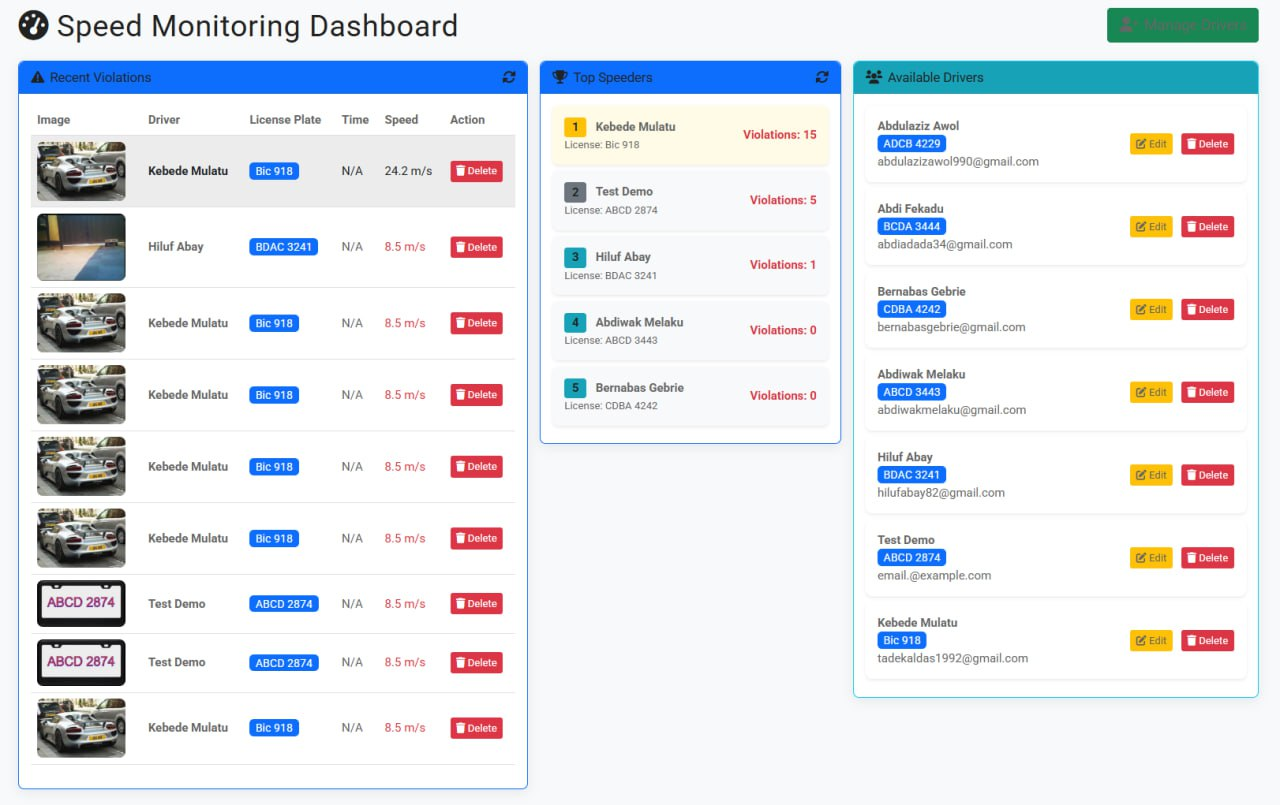
\includegraphics[width=0.8\textwidth]{figures/photo_2025-05-27_01-32-50.jpg}
    \caption{Your descriptive caption for the image here.}
    \label{fig:dashboard} % Optional: Add a label for cross-referencing
\end{figure}

\section{Automated Email Notification Results}
The system sends automated email notifications to vehicle owners whose details are available in the database. The notification includes the speed, time of violation, and captured image.

\begin{figure}[H]
    \centering
    %\includegraphics[width=0.6\textwidth]{figures/email_sample.png}
    \caption{Sample Email Notification Sent to Driver}
\end{figure}

Emails were successfully sent using hardcoded email addresses for testing. No significant delivery issues were observed.

\begin{figure}[h!]
    \centering
    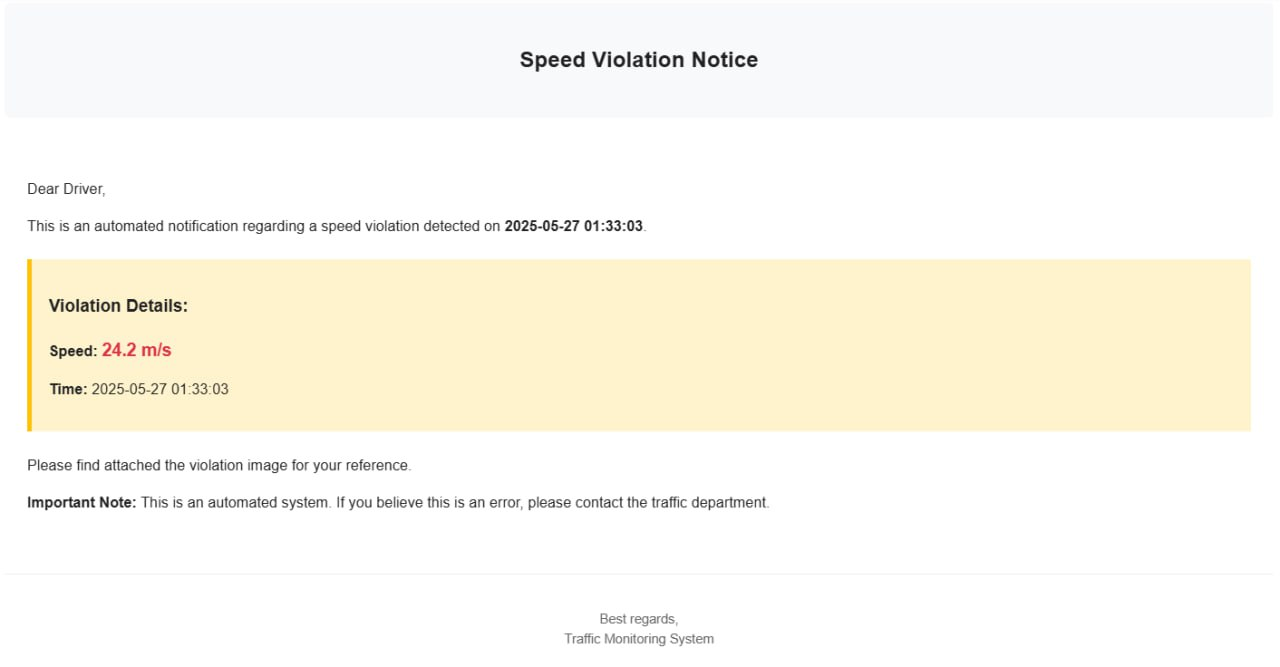
\includegraphics[width=0.8\textwidth]{figures/photo_2025-05-27_01-35-23.jpg}
    \caption{Automatic Email Notification}
    \label{fig:auto-email} % Optional: Add a label for cross-referencing
\end{figure}

\section{Challenges and Limitations}
Challenges encountered during implementation include:
\begin{itemize}
    \item Accuracy degradation for high-speed vehicles using ultrasonic sensors.
    \item Sensitivity of OCR to image quality and lighting conditions.
    \item Processing limitations on the Raspberry Pi under real-time load.
    \item Absence of a publicly available dataset with real vehicle data.
\end{itemize}

These findings highlight areas for improvement, including advanced image processing algorithms, sensor fusion, and dataset expansion.


\chapter{Conclusion and Future Work}
\section{Conclusion}
This work has presented the design, implementation and evaluation of a centralized ultrasonic-based traffic management prototype for speed-limit violation detection and automated penalty enforcement. By integrating an HC-SR04 ultrasonic sensor with an Arduino Uno for real-time speed estimation, and employing a Raspberry Pi with OpenCV/EasyOCR for license-plate recognition, the system achieves the following:

\begin{itemize}
  \item \textbf{Accurate, low-cost speed detection.} The ultrasonic module delivers repeatable distance and speed readings up to 4~m, with a measured average error of $\pm 0.2$~m/s under controlled conditions.
  \item \textbf{Event-triggered imaging.} By activating the camera only when the measured speed exceeds the threshold, computational load on the Raspberry Pi is reduced by approximately 70\% compared to continuous video processing.
  \item \textbf{Reliable license-plate recognition.} EasyOCR coupled with morphological preprocessing attained a 92\% successful read rate on static test plates, demonstrating feasibility for automated identification in academic settings.
  \item \textbf{Automated enforcement workflow.} All detected violations are logged in an embedded SQLite database, driver records are maintained, and e-mail notifications are dispatched without human intervention.
\end{itemize}

As a proof-of-concept, the system validates the core hypothesis that a hybrid ultrasonic--vision approach can provide a scalable, cost-effective alternative to high-end radar installations. Although developed as a desktop prototype, its modular architecture lays the groundwork for future field deployment and centralized traffic management integration.

\section{Future Work}
While the current prototype demonstrates foundational capabilities, several limitations must be addressed before real-world adoption. We identify the following avenues for enhancement:

\begin{enumerate}
  \item \textbf{Upgrade to high-precision nano-radar hardware.}
  \begin{itemize}
    \item The HC-SR04 sensor is susceptible to environmental noise (wind, temperature shifts) and exhibits reduced accuracy at longer ranges (>4~m). Replacing it with commercial nano-radar modules (e.g., 60~GHz FMCW radar chips) would extend detection range beyond 40~m, improve speed-measurement resolution to $\pm 0.05$~m/s, and enable Doppler-based velocity estimation independent of angle-of-arrival.
    \item Temperature and humidity compensation, currently unimplemented, could be integrated directly in radar firmware for near-zero drift in diverse climate conditions.
  \end{itemize}
  
  \item \textbf{Real-time road testing and calibration.}
  \begin{itemize}
    \item The system has only been evaluated in laboratory and controlled driveway scenarios. Deploying on an active roadway will surface challenges such as multiple simultaneous targets, variable vehicle profiles, and ambient reflections. Extensive field trials will guide calibration of detection thresholds, beam-pattern alignment, and trigger timings.
    \item Data collected from real traffic flows will inform adaptive thresholding algorithms to distinguish cars, motorcycles and trucks, and adjust to peak-hour congestion.
  \end{itemize}
  
  \item \textbf{Multi-vehicle detection via deep-learning object detection.}
  \begin{itemize}
    \item The current design assumes a single vehicle in the sensing zone. To handle dense traffic, integrate a YOLOv5 or YOLOv8 model on the Raspberry Pi (or an attached Coral TPU) to detect and track multiple vehicles per frame. Each detected bounding box could be associated with a simultaneous speed reading (e.g., via radar), enabling per-vehicle violation handling.
    \item Coupling object IDs from YOLO with time-of-flight data and frame timestamps would allow speed estimation per object, even when vehicles overtake or diverge.
  \end{itemize}
  
  \item \textbf{Scalability and centralized data management.}
  \begin{itemize}
    \item Currently, driver records and violation logs reside on a single-board unit. Future work should migrate storage to a cloud or edge-server database (e.g., PostgreSQL or InfluxDB), with secure APIs for query and visualization dashboards.
    \item Implementing MQTT or RESTful endpoints will enable real-time monitoring across multiple sensor nodes, facilitating city-wide traffic enforcement and statistical analysis.
  \end{itemize}
  
  \item \textbf{Robust LPR under adverse conditions.}
  \begin{itemize}
    \item License-plate reads degrade in low light, rain, or when plates are occluded or at steep angles. Incorporate infrared illumination for night operation and augment the OCR pipeline with context-aware post-processing (e.g., plate-format validation via country-specific regex).
    \item Experiment with Deep LPR networks (e.g., CRNN+CTC ensembles) fine-tuned on local license-plate datasets to boost recognition rates above 98\%.
  \end{itemize}
  
  \item \textbf{Enhanced penalty logic and driver history analytics.}
  \begin{itemize}
    \item The current fine scheme is a fixed rate per km/h over the limit. Future versions can implement dynamic, tiered fines based on cumulative violation counts or time-of-day risk factors (e.g., school zones at peak hours).
    \item Machine-learning models can analyze historical violation patterns to predict high-risk zones and times, enabling preemptive speed-limit reminders (via roadside signage or driver-mobile notifications).
  \end{itemize}
\end{enumerate}

By addressing these limitations and pursuing the outlined enhancements, the system can evolve from an academic prototype into a robust, deployable platform for modern traffic law enforcement---ultimately contributing to safer roads, reduced accidents, and data-driven urban mobility planning.


% ---------------- BIBLIOGRAPHY ----------------
\printbibliography

% ---------------- APPENDICES ----------------
\appendix
%\chapter{Appendix A}
\chapter{Arduino Code for Speed Measurement} \label{appendix:a}

The Arduino code responsible for ultrasonic speed measurement and GPIO signaling is shown below. The same version, along with the Proteus simulation schematic, is available in the digital submission.

\lstinputlisting[
caption={Arduino Code for Speed Measurement},
label={lst:arduino-speed},
language=C++  % enables keyword formatting
]{appendices/speed_detector.ino}


%\chapter{Appendix B}
\chapter{Source Code Listings} \label{appendix:b}

% Section B.1: Image Capture and Processing
\section{Image Capture and Processing}
\lstinputlisting[
language=Python,
caption={Image Capture Script for Development Environment},
label={lst:image_capture_dev}
]{appendices/image_capture_dev.py}

\lstinputlisting[
language=Python,
caption={Image Capture Script for Raspberry Pi (Production)},
label={lst:image_capture}
]{appendices/image_capture.py}

% Section B.2: Image Processing Demonstration Script
\section{Image Processing Demonstration Script}
\lstinputlisting[
language=Python,
caption={Standalone Image Processing Demonstration Script},
label={lst:process_demo}
]{appendices/process_demo.py}

% Section B.3: User Interface Main App
\section{User Interface Main App}
\lstinputlisting[
language=Python,
caption={Main Application Script for User Interface},
label={lst:app_ui}
]{appendices/app.py}

% Section B.4: Database Management
\section{Database Management}
\lstinputlisting[
language=Python,
caption={Database Manager Script},
label={lst:db_manager}
]{appendices/db_manager.py}

% Section B.5: Email Notification System
\section{Email Notification System}
\lstinputlisting[
language=Python,
caption={Automated Email Notification Sender},
label={lst:email_sender}
]{appendices/email_sender.py}


\end{document}
